\chapter[Sample Selection Bias]{Sample Selection Bias}
\label{ch:sample-selection-bias}\index{sample selection bias|(}

    In traditional statistics, the algorithms assume that the the data samples are being drawn in line with the same distribution, and different classes and values of data should appear with roughly the same frequency that they actually occur in the real world. However, this is rarely the case and results in the data becoming biased, meaning that the method of sample collection favours a particular type of data, skewing the distribution of the values \citep{CuddebackEtAl2004}.

    There could be a number of reasons as to why this bias occurs \citep{Tommasi2017}, such as:

    \begin{enumerate}
        \item It might be costly or unpractical to collect certain data.
        \begin{itemize}
        	\item For example, measuring spending habits of large groups of people would be cumbersome, and these people may not necessarily give accurate information.
        \end{itemize}
        \item The entity collecting the data only has access to data belonging to a particular class.
        \begin{itemize}
        	\item For example, if a doctor only has access to patients that are sick, a large portion of the sample would represent sick patients, whereas in relation to the total population the number of sick people would be relatively much smaller.
		\end{itemize}        
        \item Confirmation bias\index{sample selection bias!confirmation bias}, whereby people tend to recall only examples that confirm their existing beliefs.
        \item Incorrect sampling techniques \citep{Marshall1996}, such as sampling from the top of a list instead of randomly
        \item Sampling using results generated from another process.
        \begin{itemize}
        	\item For example, if a system is being trained on detecting fraudulent transactions, and some of these transactions were classified incorrectly by another process, then the model will be trained on false data.   
   		\end{itemize}
    \end{enumerate} 
    
    
    An interesting example that tends to happen within Maltese populations is that related with politics. When a political party passes an online poll regarding a particular issue, the results always tend to be in its favour. This stems from the fact that even though the poll is open to the general public, the outreach of the poll would be much more inclined to reach people within the party - they would have subscribed to social media and news pages, and would regularly follow or check up on their articles and news.
    
    \section{False Information created by Selection Bias}
    
	Having selection bias within a dataset can create false information which does not exist in the actual population, and can lead to inaccurate estimates of the relationships between variables \citep{CuddebackEtAl2004}.
	
	For example, assume a college accepts students that either have high math skills or high science skills. Therefore if a student in this college does not have high math skills, then he must instead have high science skills. This means that a negative correlation between maths and science skills has been created, which does not represent the actual population.
	
	
	\section{How To Prevent Selection Bias}
	
	When collecting a sample of data, one should be attentive in order to prevent selection bias occurring in the dataset. This step of preventing bias is important as not only could it skew the results, but might end up rendering the analysis and conclusions gained from the dataset as useless.
	
	\subsection{Stratified Sampling}\index{sample selection bias!stratification}
	
	This process involves splitting the population into sub-populations before selecting, in order to ensure that an adequate number from each group is selected. For example, splitting a population into age categories and selecting a number from each category \citep{KrautenbacherEtAl2017}
	
	\begin{figure}[hbt!]
	\centering
  		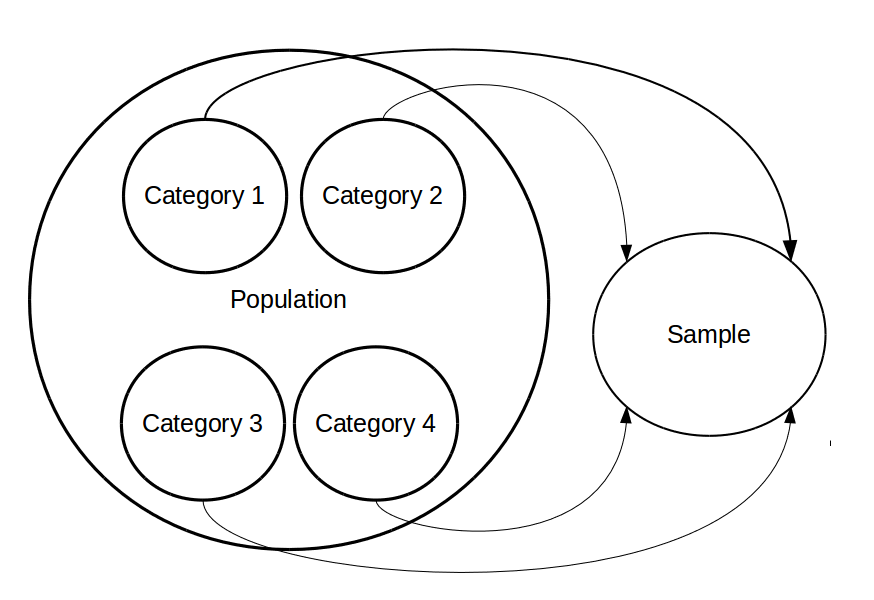
\includegraphics[width=0.88\linewidth]{graphics/sample_selection_bias/Stratified_Diagram.png}
  		\caption{Stratified sampling: splitting the population into categories and selecting accordingly}
  		\label{fig:stratified-sampling}
	\end{figure}
	
	
	\subsection{Not Self Selecting}
	
	Draw from a sample that is not self selecting. If the sample is self-selected, people who are willing to volunteer may share similar characteristics (such as be more outgoing and extroverted), which will create a bias.
	
	\subsection{Analyze Dropouts}	
	
	Determine factors affecting drop outs and establish that no differences exist between participants and non-participants. If those refusing to participate all belong to a certain category, this will create a bias and results need to be corrected to account for these differences \citep{AlonsoEtAl2006}.
	
	\subsection{Sufficient Sample Size}
	
	Ensure a large enough sample size. If the sample size is too small, it will make it more difficult to create an accurate representation.
	
	
	\section{Detecting Selection Bias within a Dataset}
	
	Once data has been collected, or when working on a dataset gained from a different source, it is important to determine whether any sample selection bias exists within the dataset before performing analysis or drawing any conclusions. The processes mentioned below are some methods which can be useful in the detecting such bias.
	
	\subsection{Comparing Distributions}\index{sample selection bias!distribution}
	
	If it is possible to capture information regarding distribution about the whole population, one may then compare this with the sample population. If the distribution if drastically different, it will indicate that a sample selection bias is present.
	
	\begin{marginfigure}
	\centering
  		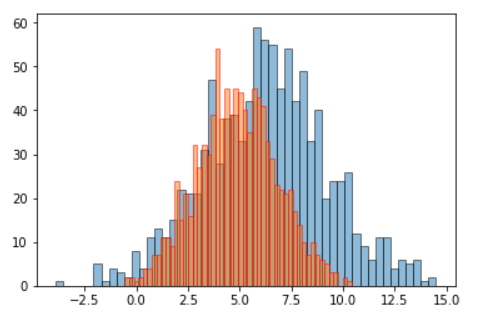
\includegraphics[width=\linewidth]{graphics/sample_selection_bias/Distributions.png}
  		\caption{Comparing Distributions}
  		\label{fig:comparing-distributions}
	\end{marginfigure}

As a simple example, if the total population contains 50\% males and females, whilst your sample contains 75\% males and 25\% females, it will indicate a selection bias which will skew the results.

Techniques exist to allow the comparison of distributions and measuring the the difference, such as Bayesian Analysis, Kolmogorov--Smirnov test or Chi-Squared test. \citep{GriffinEtAl2013}

	\subsection{Two Step Estimator}\index{sample selection bias!two-step estimator}
	
	This method, as defined by \citet{Heckman1979}, comprises the use of two multiple regression models:
	
	\begin{itemize}
		\item One model is used to examine the interest of the study.
		\item The other regression model is used to detect selection bias and to statistically correct the substantive model. The independent variable could be set to represent participation. The  dependent variable could represent different related statistics.
	\end{itemize}
	
	\subsection{Two Step Estimator Example}
	
	Imagine a survey aiming to collect information about European citizens quality of life. This would include factors such as job status, salary, level of eduction, country GDP, amongst others.
	
The first model would simply use these factors to create a model determining each citizens overall quality of life.

The second model would then measure relationships between participation and other variables. If for example a positive correlation exists between level of education and participation, then a bias in the study has occurred whereby those with a lower level of eduction are being underrepresented.

	\begin{figure}[hbt!]
	\centering
  		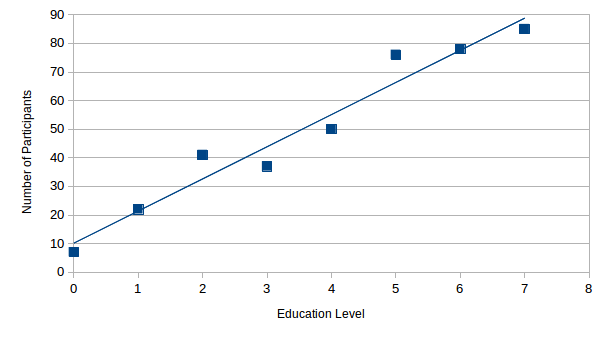
\includegraphics[width=0.88\linewidth]{graphics/sample_selection_bias/Education_Correlation_Graph.png}
  		\caption{Two Step Estimator: Using regression models to determine correlations between participants and non-participants}
  		\label{fig:correlation}
	\end{figure}
	
	\section{How to Deal With Selection Bias}
	
	If presented with a dataset which contains selection bias but which cannot be changed or modified due to a number of reasons, then adequate measures should be taken to either mitigate the bias or account for it in the results.
	
	
	\subsection{Post-stratification}\index{sample selection bias!stratification}
	
	In an attempt to make the results more representative of the total population, higher weightings are given to the lower class. If say a sample contains 25\% women, but the general population has 50\%, then you could adjust the estimates by assigning women in the sample higher weights \citep{HoltSmith1979}.
	
As explained by \citet{CortesEtAl2008}, the generalization error \textit{R} on the newly weighted sample is defined as follows:
	
	\begin{equation}\label{weighted_error_function}
    R(h) = \sum_{i=1}^m w_ic(h,z_i)
	\end{equation}
	
	Where \textit{m} is the number of samples, \textit{h} is the error value, \textit{w} is the weight, \textit{c} is the cost function and \textit{z} is the sample value.
	
	\subsection{Synthetic Minority Oversampling TEchnique (SMOTE)}\index{sample selection bias!smote}
	
	Another method of dealing with imbalanced classes is that of generating synthetic data that closely resembles the underrepresented class. In cases where the majority class greatly outweigh the minority class, having a larger dataset that more closely resembles the minority class will balance the results generated.
	
	The way this process works is that new samples are created by finding the midpoint between the line segments joining the existing samples within the minority class.	
	
	\begin{figure}
	\centering
  		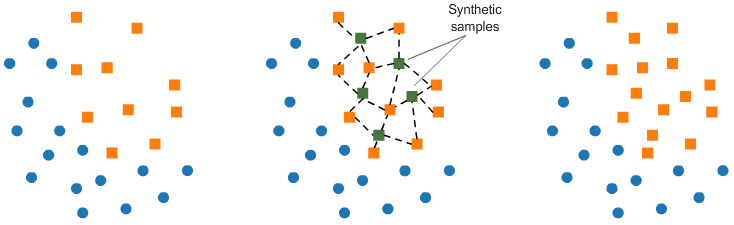
\includegraphics[width=0.88\linewidth]{graphics/sample_selection_bias/Smote.png}
  		\caption{SMOTE: generating synthetic samples of the minority class}
  		\label{fig:correlation}
	\end{figure}
	
	SMOTE may also create certain drawbacks. Since the synthetic results are generated on a small set of existing features, it may create an overfitting scenario which might not be able to correctly classify the true outlier nature of the minority class.
	SMOTE might also skew the distribution of the dataset which could affect certain analysis. The large addition of additional samples could also slow down learning speed.\citep{Weiss2007}
	
Studies seem to have shown that using SMOTE techniques to over-represent the minorty class, as opposed to under-representing the majority class by selecting fewer, tends to perform better \citep{ChawlaEtAl2002}. 


	\subsection{Applicability Disclosure}
	
	Giving full disclosure: If it is not possible to eliminate the selection bias from the dataset, then it is important to fully disclose who exactly the results and knowledge gained from the data are applicable to.

